\documentclass{beamer}
\usetheme{Madrid} % Change the theme if needed
\usepackage[autostyle=true]{csquotes}  % Language-aware quoting, required by biblatex
\usepackage{booktabs} % Add this to your LaTeX preamble if not already present
\usepackage[
    backend=biber,
    style=authoryear,
    natbib=true,           % Enable \citep / \citet commands
    uniquename=false,
    uniquelist=false,
    maxcitenames=3,        % "Author et al." when > 3 authors in a citation
    maxbibnames=999,        % Show all authors in the reference list
    giveninits=true,
    dashed=false,
    sorting=nyt,
    url=false,
    doi=false,
    isbn=false,
    eprint=false
]{biblatex}

\DeclareNameAlias{sortname}{family-given}   % Sort bibliography by last name
\DeclareDelimFormat{nameyeardelim}{\addcomma\space}
\renewbibmacro*{date+extrayear}{%
    \setunit{\addcomma\space}%
    \printtext[parens]{%
        \printfield{labelyear}%
        \printfield{extrayear}}}
\DeclareFieldFormat{sentencecase}{#1}
\renewcommand{\newunitpunct}{\addcomma\space}
\renewbibmacro{in:}{}
\DeclareFieldFormat[
    article,
    inbook,
    incollection,
    inproceedings,
    misc,
    online,
    report,
    thesis,
    unpublished
]{title}{\textquotedblleft#1\textquotedblright}
\addbibresource{references.bib}

% Italicise "et al." in citations
\usepackage{xpatch}
\xpatchbibmacro{name:andothers}{%
    \bibstring{andothers}%
}{%
    \bibstring[\emph]{andothers}%
}{}{}
\usepackage{tikz}
% \usepackage{natbib} % Enables Harvard-style citations
% \bibliographystyle{apalike}  
% \usepackage[labelfont=bf,labelsep=space]{caption}
% \captionsetup[figure]{name=Fig.}

\title{DYNAMIC CONTEXT-AWARE TRIES FOR KNOWLEDGE GRAPH-CONSTRAINED LARGE LANGUAGE MODEL GENERATION}
\author{BERNARD KIRK ADJANOR KATAMANSO
\newline ERICA AMONOR
\newline JOSEPH OSEI NYARKO
\newline JESSICA AFUA ETORNAM NSAFOAH
\newline
\newline Supervised By: DR ERIC AFFUM}
\institute{University of Mines and Technology \\ Faculty of Computing and Mathematical Science \\ Computer Science and Engineering Department}
\logo{
\includegraphics[height =1.5 cm]{WhatsApp Image 2025-03-11 at 11.07.51_bbf10778.jpg}}
\date{ July ,2026}

\begin{document}

% Title Slide
\begin{frame}
    \titlepage
\end{frame}

% Presentation Outline
\begin{frame}{Presentation Outline}

    \begin{enumerate}
        \item Introduction
        \item Statement of Problem
        \item Aims and Objectives
        \item Methodology
        \item Results and Evaluation
        \item Discussion and Contribution
        \item Recommendation
        \item References
    \end{enumerate}
\end{frame}

% Introduction
\begin{frame}{Introduction}

    \begin{itemize}
        \item LLMs are now central to AI applications, but they often hallucinate and produce factually incorrect outputs \citep{brown2020language}
        \vspace{0.3cm}
        \item KGQA demands answers that follow real graph structure \citep{he2021improving,lan2022survey}; RAG and constrained decoding both try to anchor generation to verified facts \citep{lewis2020rag,decao2021autoregressive,willard2023outlines,geng2023grammarconstrained}
        \vspace{0.3cm}
        \item Existing constrained decoding (GCR, DoG) guarantees validity, not relevance, leaving room for technically correct but irrelevant paths \citep{geng2023grammarconstrained,li2024-decoding-on-graphs}
    \end{itemize}
\end{frame}

% Problem Statement
\begin{frame}{Statement of Problem}

    \begin{itemize}
        \item GCR's trie is built before decoding starts, so it can't adapt to the question's intent or the evolving reasoning chain \citep{luo2025-graph-constrained-reasoning}
        \vspace{0.3cm}
        \item This forces the LLM back onto internal knowledge to filter out structurally valid but semantically irrelevant paths \citep{li2024-decoding-on-graphs,luo2025-graph-constrained-reasoning}
    \end{itemize}
\end{frame}

% Objectives
\begin{frame}{Project Objectives(1/3)}

    \begin{itemize}
        \item Characterize the constraint permissiveness problem by measuring the Semantic Irrelevance Ratio (SIR) of GCR's static KG-Tries on WebQSP, stratified by hop depth
        \vspace{0.3cm}
        \item Design a symbolic constraint oracle (TypeOracle) using a range gate and a type gate to filter candidate KG paths, avoiding the cost and threshold sensitivity of embedding-based approaches
    \end{itemize}
\end{frame}

\begin{frame}{Project Objectives(2/3)}

    \begin{itemize}
        \item Implement DCA-Trie v1, a static filtering variant applied at trie-construction time, keeping the false negative rate on gold paths below 5\% on the WebQSP validation set
        \vspace{0.3cm}
        \item Implement DCA-Trie v2, a dynamic variant that updates the trie after each committed triplet, conditioned on the question and the partial reasoning chain
    \end{itemize}
\end{frame}

\begin{frame}{Project Objectives(3/3)}

    \begin{itemize}
        \item Evaluate DCA-Trie v1 and v2 against the GCR baseline and an unconstrained chain-of-thought baseline on WebQSP, measuring Hits@1, F1, structural faithfulness, SIR, and average trie size
    \end{itemize}
\end{frame}

% Tools and Facilities to Be Used
\begin{frame}{Tools and Facilities Used (1/2)}
\textbf{Software Tools:}
    \begin{itemize}
        \item Python
        \item HuggingFace Transformers
        \item GCR Framework
        \item Sentence-transformers (all-MiniLM-L6-v2)
        \item PyTorch
        \item NetworkX
        \item Freebase (WebQSP and CWQ Datasets)
        \item NVIDIA GeForce RTX 4090 (24 GB)
    \end{itemize}
\end{frame}

\begin{frame}{Tools and Facilities Used (2/2)}
\textbf{Facilities:}
    \begin{itemize}
        \item NVIDIA GeForce RTX 4090 GPU (24 GB VRAM)
        \item Online academic databases (ACM Digital Library, arXiv, Google Scholar, ACL Anthology)
    \end{itemize}
\end{frame}

% Methods to Be Used
\begin{frame}{Methods Used}

    \begin{itemize}
        \item Literature Review and Theoretical Baseline
        \item Algorithm Design
        \item Type Oracle \& Algorithm Implementation
        \item Experimental Benchmarking and Evaluation
    \end{itemize}
\end{frame}

% Scope of Work
\begin{frame}{Methodology}
\begin{figure}[h]
  \centering
  \resizebox{\textwidth}{!}{%
    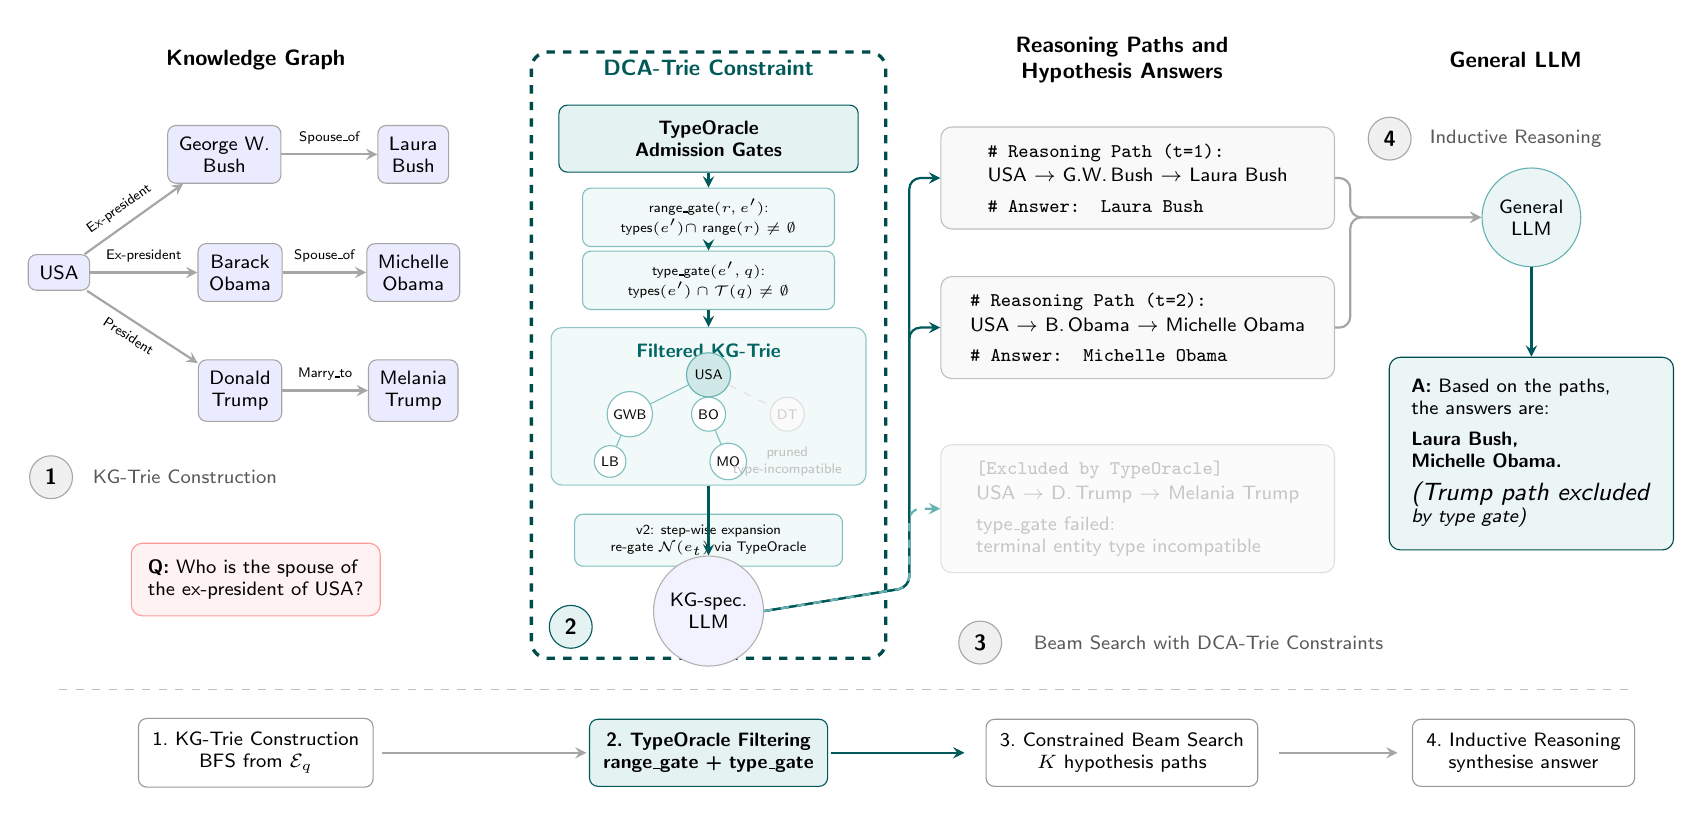
\begin{tikzpicture}[
        >=stealth, font=\sffamily,
        kgnode/.style={draw=gray!70,fill=blue!8,rounded corners=3pt,inner sep=4pt,font=\sffamily\scriptsize,align=center},
        pathbox/.style={draw=gray!50,fill=gray!5,rounded corners=4pt,inner sep=6pt,minimum width=5.0cm,align=left,font=\sffamily\scriptsize},
        ansbox/.style={draw=teal!60!black,fill=teal!8,rounded corners=4pt,inner sep=8pt,minimum width=3.0cm,align=left,font=\sffamily\scriptsize},
        stepbox/.style={draw=black!40,fill=white,rounded corners=3pt,inner sep=5pt,minimum width=2.6cm,minimum height=0.85cm,align=center,font=\sffamily\scriptsize},
        dcabox/.style={draw=teal!70!black,fill=teal!10,rounded corners=3pt,inner sep=5pt,minimum width=2.6cm,minimum height=0.85cm,align=center,font=\sffamily\scriptsize\bfseries},
        gatebox/.style={draw=teal!50,fill=teal!5,rounded corners=3pt,inner sep=4pt,font=\sffamily\tiny,align=center},
        llmcirc/.style={circle,draw=gray!60,fill=blue!5,minimum size=1.1cm,align=center,font=\sffamily\scriptsize},
        bigllm/.style={circle,draw=teal!60,fill=teal!8,minimum size=1.25cm,align=center,font=\sffamily\scriptsize},
        arr/.style={->,thick,draw=gray!70},
        tarr/.style={->,thick,draw=teal!70!black},
      ]

      % Knowledge Graph Section
      \node[font=\sffamily\footnotesize\bfseries]at(2.5,0.2){Knowledge Graph};
      \node[kgnode](usa)at(0,-2.5){USA};
      \node[kgnode](gwb)at(2.1,-1.0){George W.\\Bush};
      \node[kgnode](lb)at(4.5,-1.0){Laura\\Bush};
      \node[kgnode](bo)at(2.3,-2.5){Barack\\Obama};
      \node[kgnode](mo)at(4.5,-2.5){Michelle\\Obama};
      \node[kgnode](dt)at(2.3,-4.0){Donald\\Trump};
      \node[kgnode](mt)at(4.5,-4.0){Melania\\Trump};

      \draw[arr](usa)--node[above,sloped,font=\sffamily\tiny,pos=0.45]{Ex-president}(gwb);
      \draw[arr](usa)--node[above,font=\sffamily\tiny,pos=0.5]{Ex-president}(bo);
      \draw[arr](usa)--node[below,sloped,font=\sffamily\tiny,pos=0.45]{President}(dt);
      \draw[arr](gwb)--node[above,font=\sffamily\tiny]{Spouse\_of}(lb);
      \draw[arr](bo)--node[above,font=\sffamily\tiny]{Spouse\_of}(mo);
      \draw[arr](dt)--node[above,font=\sffamily\tiny]{Marry\_to}(mt);

      \node[draw=red!40,fill=red!5,rounded corners=4pt,inner sep=6pt,align=left,
        font=\sffamily\scriptsize,minimum width=2.9cm]
      (qbox)at(2.5,-6.4){\textbf{Q:} Who is the spouse of\\the ex-president of USA?};
      \node[circle,draw=black!35,fill=black!6,font=\sffamily\footnotesize\bfseries,inner sep=3pt]at(-0.1,-5.1){1};
      \node[font=\sffamily\scriptsize,text=black!65,align=center]at(1.6,-5.1){KG-Trie Construction};

      % DCA-Trie Constraint Section
      \draw[draw=teal!60!black,dashed,rounded corners=6pt,line width=1.2pt](6.0,0.3)rectangle(10.5,-7.4);
      \node[font=\sffamily\footnotesize\bfseries,text=teal!70!black]at(8.25,0.1){DCA-Trie Constraint};
      \node[dcabox,minimum width=3.8cm](vf)at(8.25,-0.8){TypeOracle\\Admission Gates};

      % TypeOracle gates inside the box
      \node[gatebox,minimum width=3.2cm](rg)at(8.25,-1.8){range\_gate$(r, e')$:\\types$(e') \cap$ range$(r) \neq \emptyset$};
      \node[gatebox,minimum width=3.2cm](tg)at(8.25,-2.6){type\_gate$(e', q)$:\\types$(e') \cap \mathcal{T}(q) \neq \emptyset$};

      \node[draw=teal!45,fill=teal!5,rounded corners=4pt,minimum width=4.0cm,minimum height=2.0cm](triebox)at(8.25,-4.2){};
      \node[font=\sffamily\scriptsize\bfseries,text=teal!80!black]at(8.25,-3.5){Filtered KG-Trie};

      \node[circle,draw=teal!60,fill=teal!18,inner sep=2pt,font=\sffamily\tiny](tr)at(8.25,-3.8){USA};
      \node[circle,draw=teal!50,fill=white,inner sep=1.5pt,font=\sffamily\tiny](tn1)at(7.25,-4.3){GWB};
      \node[circle,draw=teal!50,fill=white,inner sep=1.5pt,font=\sffamily\tiny](tn2)at(8.25,-4.3){BO};
      \node[circle,draw=gray!25,fill=gray!4,inner sep=1.5pt,font=\sffamily\tiny,text=gray!40](tn3)at(9.25,-4.3){DT};
      \node[circle,draw=teal!50,fill=white,inner sep=1.5pt,font=\sffamily\tiny](tl1)at(7.0,-4.9){LB};
      \node[circle,draw=teal!50,fill=white,inner sep=1.5pt,font=\sffamily\tiny](tl2)at(8.5,-4.9){MO};

      \draw[teal!50,thin](tr)--(tn1); \draw[teal!50,thin](tr)--(tn2);
      \draw[gray!25,thin,dashed](tr)--(tn3);
      \draw[teal!50,thin](tn1)--(tl1); \draw[teal!50,thin](tn2)--(tl2);
      \node[font=\sffamily\tiny,text=gray!50,align=center]at(9.25,-4.9){pruned\\type-incompatible};

      \node[gatebox,minimum width=3.4cm]at(8.25,-5.9){v2: step-wise expansion\\re-gate $\mathcal{N}(e_t)$ via TypeOracle};
      \node[llmcirc](kgllm)at(8.25,-6.8){KG-spec.\\LLM};

      \draw[tarr](vf)--(rg);
      \draw[tarr](rg)--(tg);
      \draw[tarr](tg)--(triebox.north);
      \draw[tarr](triebox.south)--(kgllm);

      \node[circle,draw=teal!70!black,fill=teal!10,font=\sffamily\footnotesize\bfseries,inner sep=3pt]at(6.5,-7){2};

      % Reasoning Paths and Hypothesis Answers Section
      \node[font=\sffamily\footnotesize\bfseries,align=center]at(13.5,0.2){Reasoning Paths and\\Hypothesis Answers};
      \node[circle,draw=black!35,fill=black!6,font=\sffamily\footnotesize\bfseries,inner sep=3pt]at(11.7,-7.2){3};
      \node[font=\sffamily\scriptsize,text=black!65]at(14.6,-7.2){Beam Search with DCA-Trie Constraints};
      \node[pathbox](p1)at(13.7,-1.3){%
        \texttt{\# Reasoning Path (t=1):}\\[1pt]
        USA $\to$ G.W.\,Bush $\to$ Laura Bush\\[3pt]
        \texttt{\# Answer: Laura Bush}};
      \node[pathbox](p2)at(13.7,-3.2){%
        \texttt{\# Reasoning Path (t=2):}\\[1pt]
        USA $\to$ B.\,Obama $\to$ Michelle Obama\\[3pt]
        \texttt{\# Answer: Michelle Obama}};
      \node[pathbox,draw=gray!25,fill=gray!3,text=gray!45](p3)at(13.7,-5.5){%
        \texttt{[Excluded by TypeOracle]}\\[1pt]
        USA $\to$ D.\,Trump $\to$ Melania Trump\\[3pt]
        type\_gate failed:\\
        terminal entity type incompatible};

      \draw[tarr,rounded corners](kgllm.east)-- (10.8,-6.5) |- (p1.west);
      \draw[tarr,rounded corners](kgllm.east)-- (10.8,-6.5) |- (p2.west);
      \draw[tarr,dashed,draw=teal!60,rounded corners](kgllm.east)-- (10.8,-6.5) |- (p3.west);

      % General LLM Section
      \node[font=\sffamily\footnotesize\bfseries]at(18.5,0.2){General LLM};
      \node[bigllm](gllm)at(18.7,-1.8){General\\LLM};
      \node[ansbox](ans)at(18.7,-4.8){%
        \textbf{A:} Based on the paths,\\
        the answers are:\\[3pt]
        \textbf{Laura Bush,}\\
        \textbf{Michelle Obama.}\\[4pt]
        \small\textit{(Trump path excluded}\\
        \textit{by type gate)}};
      \node[circle,draw=black!35,fill=black!6,font=\sffamily\footnotesize\bfseries,inner sep=3pt]at(16.9,-0.8){4};
      \node[font=\sffamily\scriptsize,text=black!65]at(18.5,-0.8){Inductive Reasoning};

      \draw[arr,rounded corners](p1.east) -| (16.4,-1.8) -- (gllm.west);
      \draw[arr,rounded corners](p2.east) -| (16.4,-1.8) -- (gllm.west);
      \draw[tarr](gllm)--(ans);

      % Footer Steps Section
      \draw[gray!50,dashed](0,-7.8)--(20.0,-7.8);
      \node[stepbox]at(2.5,-8.6){1.\ KG-Trie Construction\\BFS from $\mathcal{E}_q$};
      \node[dcabox]at(8.25,-8.6){2.\ TypeOracle Filtering\\range\_gate + type\_gate};
      \node[stepbox]at(13.5,-8.6){3.\ Constrained Beam Search\\$K$ hypothesis paths};
      \node[stepbox]at(18.6,-8.6){4.\ Inductive Reasoning\\synthesise answer};

      \draw[arr](4.1,-8.6)--(6.7,-8.6);
      \draw[tarr](9.8,-8.6)--(11.5,-8.6);
      \draw[arr](15.5,-8.6)--(17.0,-8.6);
    \end{tikzpicture}
  }%
  \caption[DCA-Trie System Architecture]{DCA-Trie System Architecture.}
  \label{fig:architecture}
\end{figure}
\end{frame}

% Expected Outcomes
\begin{frame}{Upgraded Constraint Specification}
    \begin{itemize}
      \item \textbf{Baseline Formalization (GCR/DoG):}
      \[
        W_{\text{val}}^{\text{GCR}}(t) = f(G, E_q)
      \]
      \item \textbf{Proposed Formalization (DCA-Trie):}
      \[
        W_{\text{val}}^{\text{DCA}}(t) = f(G, E_q, q, y_{<t})
      \]
    \end{itemize}
\end{frame}

\begin{frame}{Design Conditions}
    \begin{itemize}
      \item \textbf{Condition F (Structural Faithfulness):} $100\%$ structural grounding in KG triplets[cite: 1].
      \item \textbf{Condition R (Semantic Relevance Reduction):} Lower Semantic Irrelevance Ratio ($\overline{\text{SIR}}$)
      \item \textbf{Condition P (Recall Preservation):} False Negative Rate ($\text{FNR}$) on gold paths $< 5\%$
    \end{itemize}
\end{frame}
% Slide 1: SIR Definition & Step-Level Calculation
\begin{frame}{Diagnostic Metric: SIR Definition}
  \text{SIR} measures the fraction of structurally valid paths permitted by the constraint oracle that are semantically incompatible with the input question.

  \vspace{1em}

  \textbf{Step-Level Calculation:}
  \[
    \text{SIR}(q, t) = \frac{\sum_{p \in \mathcal{P}(q, t)} \text{irrelevant}(p, q)}{|\mathcal{P}(q, t)|}
  \]
\end{frame}

% Slide 2: Corpus-Level SIR Calculation
\begin{frame}{Diagnostic Metric: Corpus-Level SIR}
  \textbf{Corpus-Level Average:}
  \[
    \overline{\text{SIR}} = \frac{1}{|Q|} \sum_{q \in Q} \frac{1}{L_q} \sum_{t=1}^{L_q} \text{SIR}(q, t)
  \]
  
  \vspace{1em}
  
  \begin{itemize}
    \item Evaluates overall constraint search space permissiveness across the benchmark dataset.
    \item Provides a quantitative diagnostic metric independent of downstream model generation accuracy.
  \end{itemize}
\end{frame}

% Slide 3: DCA-Trie v1
\begin{frame}{Implementation Variants: DCA-Trie v1}
  \textbf{Static Symbolic Filtering}
  
  \vspace{1em}
  
  \begin{itemize}
    \item Filters BFS-enumerated paths through the Type Oracle prior to building the static prefix tree (\texttt{marisa\_trie}).
    \item Preserves static trie lookup efficiency ($O(d)$ time complexity) while pruning irrelevant branches offline.
  \end{itemize}
\end{frame}

% Slide 4: DCA-Trie v2
\begin{frame}{Implementation Variants: DCA-Trie v2}
  \textbf{Step-Wise Symbolic Expansion}
  
  \vspace{1em}
  
  \begin{itemize}
    \item Dynamically expands the trie step-by-step only when an entity token $e_t$ is committed to the reasoning path.
    \item Applies local property range and answer type gate checks to candidate neighbors $\mathcal{N}(e_t)$ during token generation.
  \end{itemize}
\end{frame}
\begin{frame}{Results}
\begin{itemize}
    \item \textbf{Sensor Performance} %The sound, temperature, and current sensors successfully captured motor operating conditions in real time with reliable accuracy.
    \vspace{5px}
    \item \textbf{Data Transmission} %Sensor data was seamlessly transmitted to ThingSpeak, enabling low-latency visualization and integration with the predictive maintenance dashboard.
     \vspace{5px}
    \item \textbf{Fault Detection} %Machine learning models (Random Forest, KNN) classified motor faults effectively, achieving high accuracy in distinguishing between normal and faulty states.
     \vspace{5px}
    \item \textbf{System Reliability} %The IoT framework provided continuous monitoring and early fault detection, reducing the likelihood of unexpected breakdowns.
     \vspace{5px}
    \item \textbf{Cost-Effectiveness} %The prototype system was low-cost compared to traditional industrial monitoring solutions, making it suitable for resource-constrained settings.
    
    \end{itemize}
\end{frame}


% Results
%\begin{frame}{Results}
\begin{frame}{Results: Comparative Evaluation}
\centering
  \small
  \resizebox{\linewidth}{!}{%
  \begin{tabular}{l c c c}
    \toprule
    \textbf{Metric / Method} & \textbf{Baseline (GCR)} & \textbf{DCA-Trie v1 (Static)} & \textbf{DCA-Trie v2 (Dynamic)} \\
    \midrule
    \textbf{Hits@1} & \textbf{91.6\%} & 86.4\% & 54.0\% \\
    \textbf{F1 Score} & \textbf{72.1\%} & 61.6\% & — \\
    \textbf{Structural Faithfulness} & \textbf{100.0\%} & \textbf{100.0\%} & \textbf{100.0\%} \\
    \textbf{Path Reduction} & 0.0\% (4.10M) & \textbf{14.5\% (3.51M)} & — \\
    \textbf{Corpus SIR} & 1.000 & \textbf{0.145} & — \\
    \textbf{Gold Path FNR} & 0.0\% & \textbf{3.3\% (Type) / 2.9\% (Range)} & — \\
    \textbf{Latency / Overhead} & 6.35s / q & \textbf{6.38s / q (+0.5\%)} & $\sim$8,000s (Partial) \\
    \bottomrule
  \end{tabular}%
  }

  \vspace{1.5em}
  \raggedright
  \footnotesize
  \textit{Evaluated on WebQSP (1,628 test queries) using Llama-3.1-8B with group-beam search ($k=10$).}
\end{frame}

% Discussion
\begin{frame}{Discussion}
\begin{itemize}
    \item IoT sensors enabled \textbf{real-time monitoring} of motor health, showing feasibility of low-cost predictive maintenance solutions.
    \item Machine learning models (Random Forest, KNN) achieved \textbf{high accuracy in fault classification}, outperforming traditional threshold-based methods.
    \item \textbf{ThingSpeak cloud platform} ensured reliable data storage and visualization, confirming open-source IoT tools are effective for predictive maintenance.
    \item The system is \textbf{cost-effective} and scalable for industries, though future work should include more sensors.
\end{itemize}
\end{frame}

%Demonstration
\begin{frame}{Demonstration}
\centering
Demonstration of project
\end{frame}

%Conclusion
\begin{frame}{Conclusion}
\begin{itemize}
    \item The IoT-based predictive maintenance system successfully monitored electric motor conditions in real-time.
    \item Machine learning models (Random Forest, KNN) effectively classified motor faults with high accuracy.
    \item The system proved cost-effective and reliable compared to traditional maintenance methods.

\end{itemize}
\end{frame}

%Recommendation
\begin{frame}{Recommendations}
\begin{itemize}
    \item Expand system with additional sensors (vibration, voltage, power factor) for enhanced fault detection.
    \item Train ML models with larger, more diverse datasets to improve generalization.
    \item Integrate edge computing to reduce cloud dependence and latency.
    \item Collaborate with industries for real-world deployment, testing, and scalability.
\end{itemize}
\end{frame}

% References
\begin{frame}{References}
    \begin{itemize}
     \item Him, S., Kim, Y., and Lee, S. (2019), "IoT-based predictive maintenance for industrial equipment", \emph{IEEE Access}, Vol. 7, pp. 113467–113477.
     \item Martins, R., Silva, A., and Pereira, J. (2020), "Condition monitoring of induction motors based on IoT and machine learning", \emph{Journal of Intelligent Manufacturing}, Vol. 31, No. 5, pp. 1119–1132.

    
    \end{itemize}
\end{frame}
% References
\begin{frame}{References}
\begin{itemize}

    \item Nangia, V., Gopal, A., and Mishra, R. (2020), "Predictive maintenance framework for electric motors using machine learning", \emph{International Journal of Prognostics and Health Management}, Vol. 11, No. 3, pp. 1–12.

          \end{itemize}
\end{frame}  

% Thank You Slide
\begin{frame}{Thank You!}
    \centering \Huge Thank You!!!
\end{frame}

\end{document}
